\documentclass[]{article}

\usepackage{amsmath}
\usepackage{amsfonts}

\usepackage{graphicx}
\graphicspath{ {./Fig/} }

% \setlength{\parindent}{0cm}
\usepackage[margin=1in]{geometry}

\bibliography{bib}

%opening
\title{Boletín Laboratorio 2}
\author{Ignacio Osorio}

\begin{document}

\maketitle

\begin{abstract}

En este laboratorio se trabajo en busquedas de texto del tipo \emph{pattern matching}. Se implemento un \emph{suffix array} \cite{SuffixArray} y una busqueda lineal para poder comparar los comportamientos de ambas formas de abordar el problema. Los datos de prueba fueron de una base de datos de texto que se puede encontrar en \emph{Pizza&Chili Corpus} \cite{data}, especificamente el archivo de 50 mbs. Se analizara tambien el tiempo de pre-procesamiento necesario para el \emph{suffix array} en función del tamaño del texto ingresado.

\end{abstract}

\section{Ejercicio 1}








Los algoritmos fueron implementados en C++ y probados en un computador personal. Las especificaciones del computador se pueden ver en la tabla \ref{tab:spec}. Todos los códigos generados para este laboratorio se encuentran adjuntos a este documento.

Los algoritmos fueron implementados de forma iterativa.

\begin{table}[]
	\centering
	\caption{Especificaciones del computador personal.}
	\label{tab:spec}
	\begin{tabular}{|c|c|c|}
		\hline
		CPU 					& RAM 			& SO 	 				\\ \hline
		Intel Core i7-7700HQ    & 16 GB        	& Windows 10 Home        \\ \hline
	\end{tabular}
\end{table}


\section{Ejercicio 2}
\subsection{Búsqueda Lineal}

Este algoritmo realizara una búsqueda lineal comenzando desde el primer elemento contenido en el vector hasta el último. Se detendrá si encuentra una ocurrencia del elemento buscado o cuando llegue al final del arreglo.

Su complejidad temporal en el peor caso es de $O(n)$, donde $n$ es el número de elementos en el arreglo. Si se realiza un análisis adaptativo considerando la posición del elemento, es fácil ver que la complejidad permanecerá lineal a esta posición, por lo que será $O(p)$, donde $p$ es la posición del elemento buscado.

Este algoritmo utiliza espacio constante para guardar una referencia a la posición del elemento. No requiere de preprocesamiento de los datos.

\subsection{Búsqueda Binaria}

Un requerimiento de este algoritmo es que los datos se encuentren ordenados previamente. La búsqueda se realiza utilizando el paradigma dividir y conquistar. Se divide el arreglo por la mitad y se compara la mediana del vector (en caso de ser número par se toma solo el elemento menor como mediana), en caso de ser el elemento se retorna la posición, en caso de ser mayor se procede a repetir el algoritmo con el sub-arreglo a la izquierda de la mediana, en caso contrario se realiza con el sub-arreglo derecho. Siempre creando los sub-arreglos de tal forma que excluyan la variable comparada.

Esto se realiza hasta que el sub-arreglo llega a tener tamaño 0 o se encuentra el elemento.

Su complejidad temporal es fácilmente calculable utilizando el teorema maestro. Como se puede ver en las siguientes ecuaciones, al tener $a=b^{c}$, la complejidad es de tipo $O(n^{c}log(n)) = O(log(n))$.

\begin{align*}
	T(n) = aT(\frac{n}{b}) + O(n^{c}) \\
	T(n) = T(\frac{n}{2}) + O(1) \\
	a = 1 \\
	b = 2 \\
	c = 0
\end{align*}

Este algoritmo tiene un análisis espacial similar al anterior, por lo que se puede decir que es $O(1)$.

La etapa de preprocesamiento tendría complejidad $O(n*log(n))$ si se utilizó algún algoritmo típico basado en comparaciones. Esta complejidad podría ser menor, dependiendo de las características de la entrada y el uso de bucket sort, radix sort u otro de la misma línea.

\subsection{Búsqueda Doblada}

Al igual que la búsqueda binaria, este algoritmo requiere que los datos se encuentren ordenados previamente para realizar la búsqueda. Además, busca integrar una cota superior logarítmica a la complejidad temporal y permitir un análisis adaptativo para mejorar el comportamiento del algoritmo para ubicaciones más cercanas del inicio.

Esto lo consigue modificando la búsqueda lineal, realizando saltos exponenciales en las posiciones $i = \{ \forall j \in \mathbf{N}_{0} : 2^j \}$. Cuando el elemento $x_{i}$ es mayor que el elemento que se está buscando, procede a realizar una búsqueda binaria en el sub arreglo de tamaño $\frac{i}{2}$ que está limitado por los elementos $x_{i-1}$ y $x_{i}$.

El análisis del peor caso dará una primera parte logarítmica en base 2 con respecto del tamaño del arreglo y la búsqueda lineal sobre el $\frac{n}{2}$ tendrá la misma complejidad, por lo tanto la complejidad total será de $O(log(n))$.

Al realizar un análisis adaptativo del algoritmo, con respecto de la posición $p$ en la que se encuentra el elemento tendremos $T(p) = \lfloor log(p) \rfloor + 1 + O(log(p))$, donde las componentes $\lfloor log(p) \rfloor + 1$ corresponden a los saltos exponenciales de la búsqueda y la componente $O(log(p))$ representa a la búsqueda binaria en el último espacio generado por el salto. Por lo tanto $T(p) \in O(log(p))$.

\section{Ejercicio 3}

Los algoritmos fueron evaluados midiendo sus tiempos de respuesta cada mil elementos insertados (variando el tamaño), usando datos aleatorios que están contenidos en el arreglo, en un rango sobre el primer tercio del arreglo, para eliminar muchos datos pequeños que arruinaban la precisión.

Además, se evaluó el comportamiento de los algoritmos frente a la posición del elemento buscado. Para esto se utilizó un arreglo de 100k elementos y se hicieron mediciones para búsquedas de datos aleatorios en ventanas de mil elementos.

Cada valor de tiempo fue calculado como el promedio de 10k mediciones.

\section{Ejercicio 4}

Se pueden observar los resultados en los gráficos \ref{fig:1} y \ref{fig:2}.

\begin{figure}[tb]
	\centering
	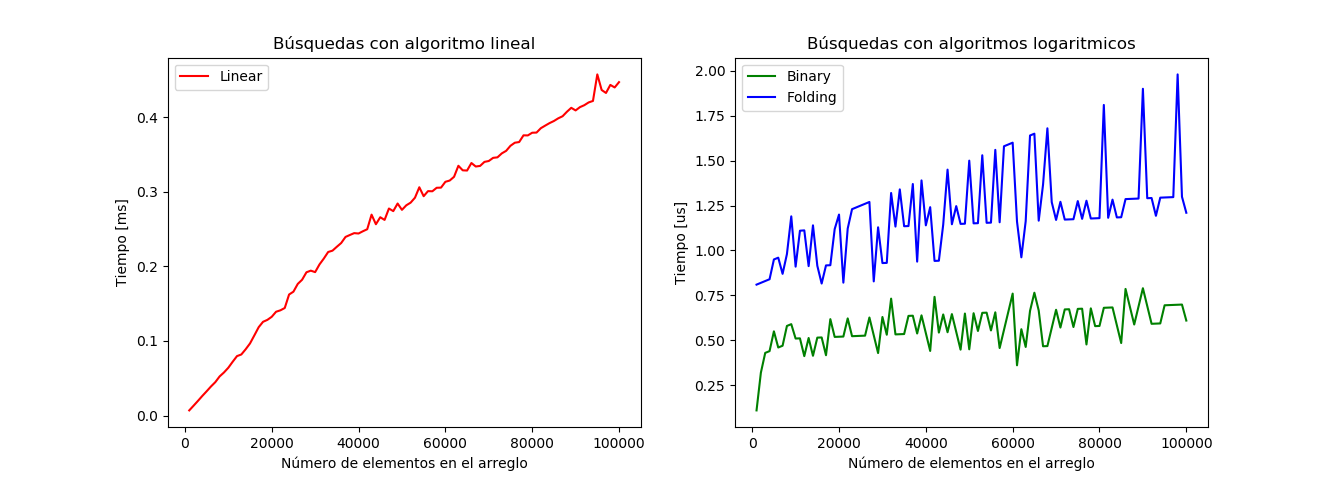
\includegraphics[width=1\textwidth]{Busqueda por tamanio}
	\caption{Tiempo que demora los algoritmos en función del tamaño del arreglo.}
	\label{fig:1}
\end{figure}

\begin{figure}[tb]
	\centering
	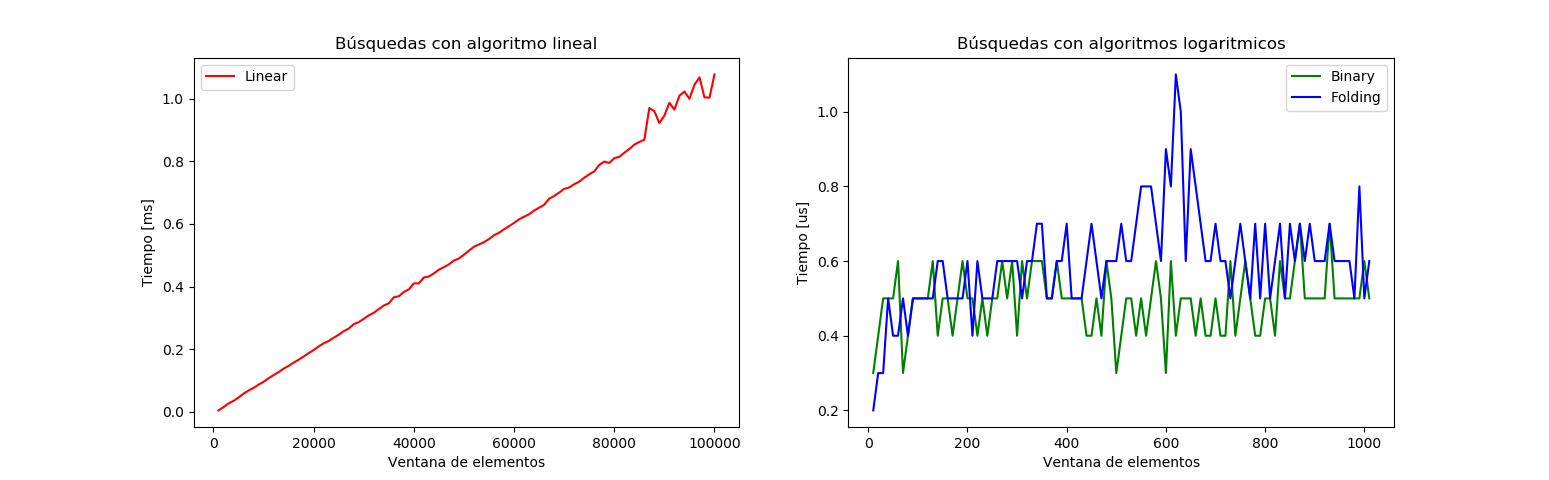
\includegraphics[width=1\textwidth]{Busqueda por p}
	\caption{Tiempo que demoran los algoritmos en función de la posición del elemento.}
	\label{fig:2}
\end{figure}

\begin{figure}[tb]
	\centering
	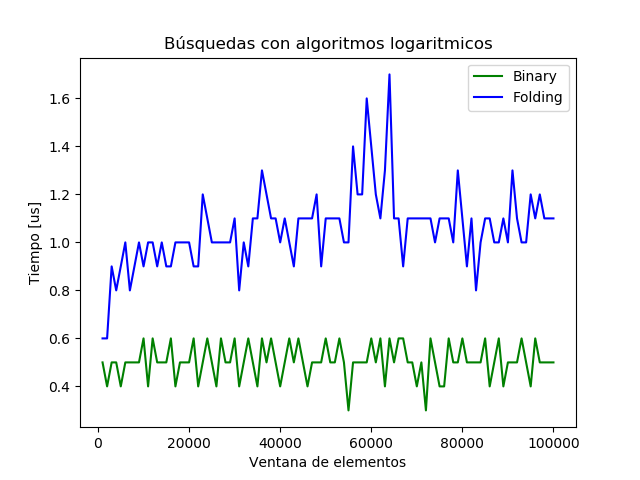
\includegraphics[width=0.7\textwidth]{Busqueda por p grande}
	\caption{Tiempo que demoran los algoritmos logaritmicos en función de posiciones grandes.}
	\label{fig:3}
\end{figure}

\section{Conclusiones}

Fue necesario restringir el dominio de los números aleatorios, para así reducir la cantidad de ruido en la toma de muestras.

Se puede observar que el comportamiento del algoritmo lineal cumple con lo esperado.

La búsqueda doblada solo logra ser más veloz que la binaria cuando los elementos se encontraban considerablemente al principio (dentro de los primeros 100 elementos), el resto del tiempo se mantenían relativamente iguales, excepto cuando $p$ tendía hasta $n$, donde el rendimiento de la búsqueda binaria estaba claramente por encima de la doblada. Esto último se puede observar en el grafico \ref{fig:3}.

A pesar de tener un análisis adaptativo mejor, la búsqueda doblada muestra ser buena solo para casos específicos donde tengamos restricciones en la entrada.


\end{document}
